\documentclass[12pt]{article}
\usepackage[utf8]{inputenc}
\usepackage{listings}
\usepackage{amsmath}
\usepackage{graphicx}
\usepackage{float}
\usepackage[margin=0.7in]{geometry}

\title{CENG478 HW1 Report}
\author{İdil Zeynep Alemdar}
\date{23.03.2019}

\begin{document}
	\begin{titlepage}
		\maketitle
	\end{titlepage}
\section*{Introduction}
In this homework, I split the task of calculating the dot product of two vectors with length 10000000 each into the number of processors. That is, if a single processor was used, all the calculation was performed as a single batch. If 2 processors were used, each process calculated dot product of 5000000 length halves and then their result is summed. If 4 processors were used, each process calculated dot product of 2500000 length quarters, and so on. I ran 30 experiments for each amount of processors, as can be seen on my code as well. While I was plotting the graph, I first calculated the average runtime for each level of parallelism.
\section*{a)}
When we inspect the vectors, we can see that there is a pattern for the first vector: \\
$2.0 - 0*0.1 = 2.0$\\
$2.0 - 1*0.1 = 1.9$\\
... \\
$2.0 - 19*0.1 = 0.1$\\
$2.0 - 0*0.1 = 2.0$\\

\noindent
recurring for every 20 iterations. For the second vector, the pattern looks like: \\
$0.1 + 0*0.1 = 0.1$\\
$0.1 + 1*0.1 = 0.2$\\
... \\
$0.1 + 19*0.1 = 2.0$\\
$0.1 + 0*0.1 = 0.1$\\
\noindent
again recurring for every 20 iterations. This situation makes our task of calculating the dot product easier: 
\begin{itemize}
	\item Multiply first 10 elements of each vector and add them together: $2.0*0.1 + 1.9*0.2+...+1.1*1.0 = 7.7$.
	\item Then, multiply this result by 2 to obtain the result for the dot product of the first 20 elements: $7.7*2 = 15.4$. 
	\item Divide 10000000 by 20 to obtain how many 20-length subvectors we have: $10000000/20 = 500000$.
	\item Multiply the latter two results to get the overall dot product: $15.4 * 500000 = 7700000$
\end{itemize}
\noindent
Hence, the result of the given task is $7700000$. Here are the results of my experiments:
\begin{table}[H]
	\begin{tabular}{|c|c|c|c|c|l|}
		\hline
		1              & 2              & 4              & 8              & 16             & 32             \\ \hline
		7700000.000132 & 7700000.000079 & 7699999.999992 & 7700000.000020 & 7699999.999980 & 7700000.000001 \\ \hline
	\end{tabular}
\end{table}

Here is the table of relative errors for each number of processors:

\begin{table}[H]
	\begin{tabular}{|c|c|c|c|c|l|}
		\hline
		1              & 2              & 4              & 8              & 16             & 32             \\ \hline
		$1.714286 * 10^{-11}$ & $1.025974 * 10^{-11}$ & $0.103896 * 10^{-11}$ & $0.259740 * 10^{-11}$ & $0.259740 * 10^{-11}$ & $0.0129870 * 10^{-11}$ \\ \hline
	\end{tabular}
\end{table}

\section*{b)}
The reason for calculating different results than the theoretical result is the floating point precision.
\section*{c)}
Below are the Time vs. Number of processors graphic and Speed Improvement vs. Number of processors graphic of the experiments:\\
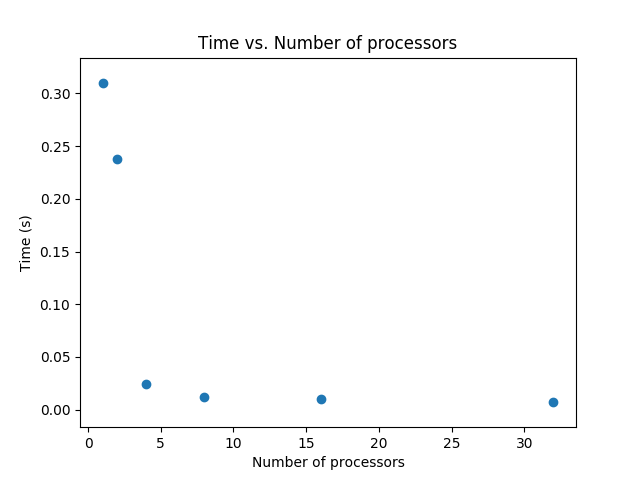
\includegraphics[scale=1]{plot1}\\
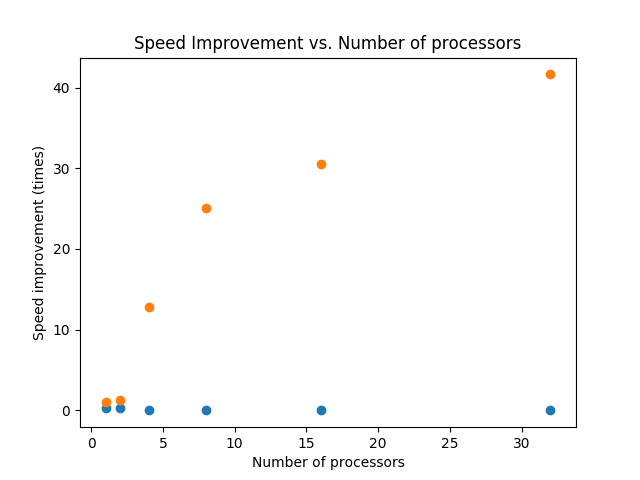
\includegraphics[scale=1]{plot2} \\
As one can see on the plots, runtime decreases as the number of processors increase. The reason behind this is of course the increase in the level of parallelism. As more processors work on the smaller parts of the same problem, the overall execution time decrease. When we inspect the plot in more detail, we observe that using 2 parallel working processors decrease the average runtime from $\approx ~0.33$ s to $\approx 0.23$ s, which means an approximately $\approx ~1.3$ times improvement on the speed. Using 4 processors, on the other hand, shows a more dramatic decrease in runtime. This time, the execution is almost 13 times faster than sequential execution. Increasing the parallelism to 8, 16 and 32 processors speed up the execution by $\approx 25$, $\approx31$, $\approx 46$ times respectively. The reason behind the fact that there is no significant difference between sequential vs 2 parallel executions while 4 or more processors decrease the execution time by multiples of 2-digit figures may be that the computational overhead of executing MPI calls such as \textit{MPI\_Reduce}. It is possible that parallel execution of two half vectors' dot product cannot compensate all-to-one reduction of their sums. When the number of processors increase, on the other hand, the sub-calculations execute much faster and hence, running time of \textit{MPI\_Reduce} will not be bottleneck anymore.
\end{document}